\documentclass[runningheads]{llncs}

\renewcommand{\labelenumii}{\theenumii}
\renewcommand{\theenumii}{\theenumi.\arabic{enumii}.}

\usepackage{graphicx}
\usepackage{hyperref} %might be better to uncomment this
\usepackage{subfig}

% Used for displaying a sample figure. If possible, figure files should
% be included in EPS format.
%
% If you use the hyperref package, please uncomment the following line
% to display URLs in blue roman font according to Springer's eBook style:
\renewcommand\UrlFont{\color{blue}\rmfamily}

\begin{document}
%
%\title{Contribution Title\thanks{Supported by organization x.}}
\title{EARIN\\Laboratory report\\EXERCISE 6: Reinforcement learning}
%
%\titlerunning{very very very }
% If the paper title is too long for the running head, you can set
% an abbreviated paper title here
\author{Bartłomiej Mastej \& Paweł Borsukiewicz}
%
\institute{Warsaw University of Technology, Warsaw, Poland}

%
\maketitle              % typeset the header of the contribution
%
%
%
%
\section{Introduction}
At the very beginning, there was prepered the environment using the openAI gym for the 'CarRacing-v0' problem. Further, there was created the Proximal Policy Optimization model which was further tuned with the usage of the Grid Search algorithm.
\section{Implementation}
First of all, there was prepared environment using the openAI gym environment. It was decided to use 'CarRacing-v0' gym instead of 'CarRacing-v1' due to high availability of libraries supporting reinforcement learning.
\subsection{Model \& learning procedure}
It was decided to use the PPO - Proximal Policy Optimization model from the $stable\textunderscore baselines3$ python module due to the ease of implementation and tuning. Furthermore, this module is implemented with the usage of the $TensorFlow$ module, hence the learning can be done with the GPU computational support. The implementation of the model creation with the parameters tuning is presented on the Fig.~\ref{fig4}. Further, there was used the $learn$ method of the module which take the timestep as the parameter. The duration of the model learning is being saved as shown on the Fig.~\ref{fig4}. Finally, there is a need to give a reward for the given simulation as well as the standard deviation. Therefore, there was used the $evaluate\textunderscore policy$ function also from the $stable\textunderscore baselines3$ module. As described in the subsection 3 the best model is being saved to a zip file.
\begin{figure}
  %width=\textwidth
  \centering
  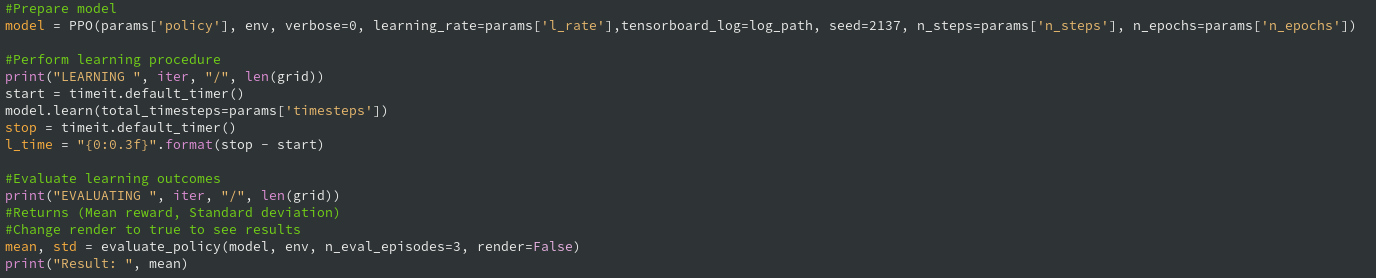
\includegraphics[width=\textwidth]{Screenshots/learn.png}
\caption{Model creation} \label{fig4}
\end{figure}


\subsection{Grid Search parameters tuning}
For the scope of tuning there was used Grid-Search process the following parameters were checked:
learning rate, policy, number of steps, number of epochs, and the timestep.
The implementation of the Grid Search was done with the usage of the $sklearn$ module and it can be seen on the Fig.~\ref{fig0}.
\begin{figure}
  %width=\textwidth
  \centering
  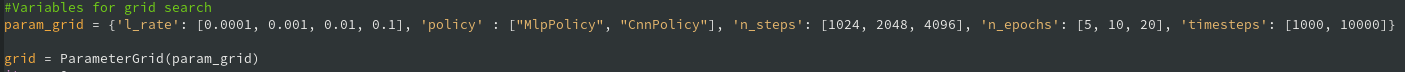
\includegraphics[width=\textwidth]{Screenshots/grid.png}
\caption{Grid Search parameters} \label{fig0}
\end{figure}
Further, there was created the main loop which iterated through all the grid search parameters:

\subsection{Results saving/loading}
Before main loop of the Grid Search was performed, there was created the $results.csv$ file that is presented on the Fig.~\ref{fig2} in which there are saved the parameters of the given iteration as well as the mean reward value and the network learning time. The save of the current results takes place just after learning outcomes are achieved Fig.~\ref{fig1}. Furthermore, it was decided to save only the best pretrained model of the given program execution as can be seen on the Fig.~\ref{fig1}. The model is being saved in the zip format. The pretrained network can be easily loaded from the file as presented on the Fig.~\ref{fig3}.
\begin{figure}
  %width=\textwidth
  \centering
  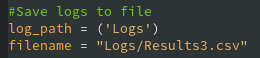
\includegraphics{Screenshots/logs.png}
\caption{Log files creation} \label{fig2}
\end{figure}

\begin{figure}
  %width=\textwidth
  \centering
  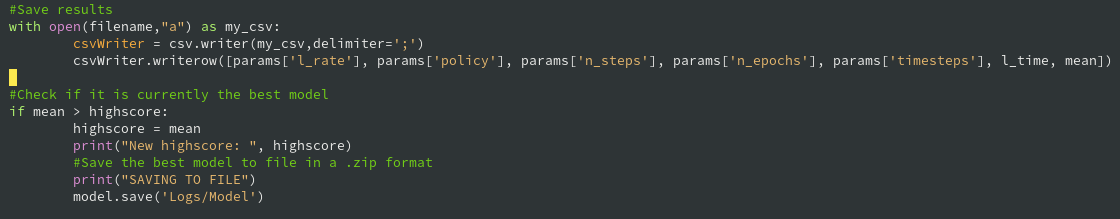
\includegraphics[width=\textwidth]{Screenshots/save.png}
\caption{Pretrained model and parameters saving} \label{fig1}
\end{figure}

\begin{figure}
  %width=\textwidth
  \centering
  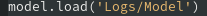
\includegraphics{Screenshots/load.png}
\caption{Loading pretrained network} \label{fig3}
\end{figure}


\section{Resuls \& conclusions}



\end{document}
